\documentclass[a4paper, 12pt]{article}
\usepackage[a4paper, total={6in, 9.5in}]{geometry} % DL: 쪽여백 조정
\usepackage{setspace} % DL: 줄간격 조정
\usepackage{graphicx} % Required for inserting images
\usepackage{kotex}
\usepackage{amsmath,amsthm,amssymb,amsfonts,mdframed}

% set indent length to zero.
\setlength{\parindent}{0pt}

\title{1113 Class Activity}
\author{박예영}

\begin{document}
\maketitle
\begin{mdframed}
Check that this theorem for cycle $C_6$.\\
\textbf{Thm)} If the eigenvalues of $A_G$ are $(k, \theta_2, \theta_3, \cdots, \theta_n)$, then the eigenvalues of $A_{\bar{G}}$ are $(n-1-k, -1-\theta_2, -1-\theta_3,\cdots,-1-\theta_n)$.
\end{mdframed}

\begin{proof}
$C_6$와 $\bar{C_6}$의 adjacency matrix $A_{C_6}$, $A_{\bar{C_6}}$는 아래와 같다.
$$A_{C_6} = \begin{pmatrix} 0 & 1 & 0 & 0 & 0 & 1 \\ 1 & 0 & 1 & 0 & 0 & 0 \\ 0 & 1 & 0 & 1 & 0 & 0 \\ 0 & 0 & 1 & 0 & 1 & 0 \\ 0 & 0 & 0 & 1 & 0 & 1 \\ 1 & 0 & 0 & 0 & 1 & 0 \\ \end{pmatrix}, A_{\bar{C_6}} = \begin{pmatrix} 0 & 0 & 1 & 1 & 1 & 0 \\ 0 & 0 & 0 & 1 & 1 & 1 \\ 1 & 0 & 0 & 0 & 1 & 1 \\ 1 & 1 & 0 & 0 & 0 & 1 \\ 1 & 1 & 1 & 0 & 0 & 0 \\ 0 & 1 & 1 & 1 & 0 & 0 \\ \end{pmatrix}$$\\
$A_{C_6}$의 eigenvalue들은 $(2, 1, 1, -1, -1, -2)$이고, $A_{\bar{C_6}}$의 eigenvalue들은 $(3, -2, -2, 0, 0, 1)$이므로 위의 정리가 잘 성립함을 확인할 수 있다.\\
\newpage
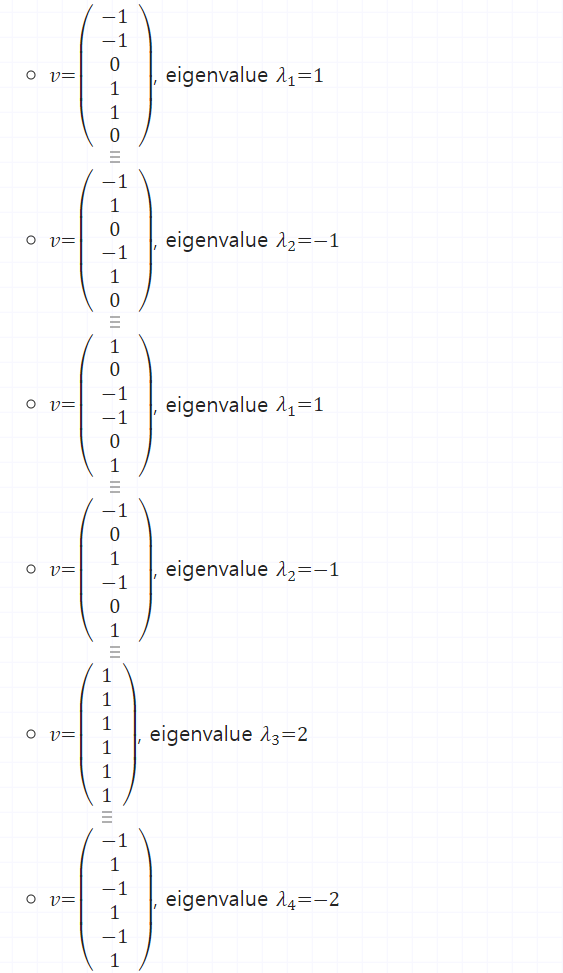
\includegraphics[width=1\linewidth]{image.png} \\
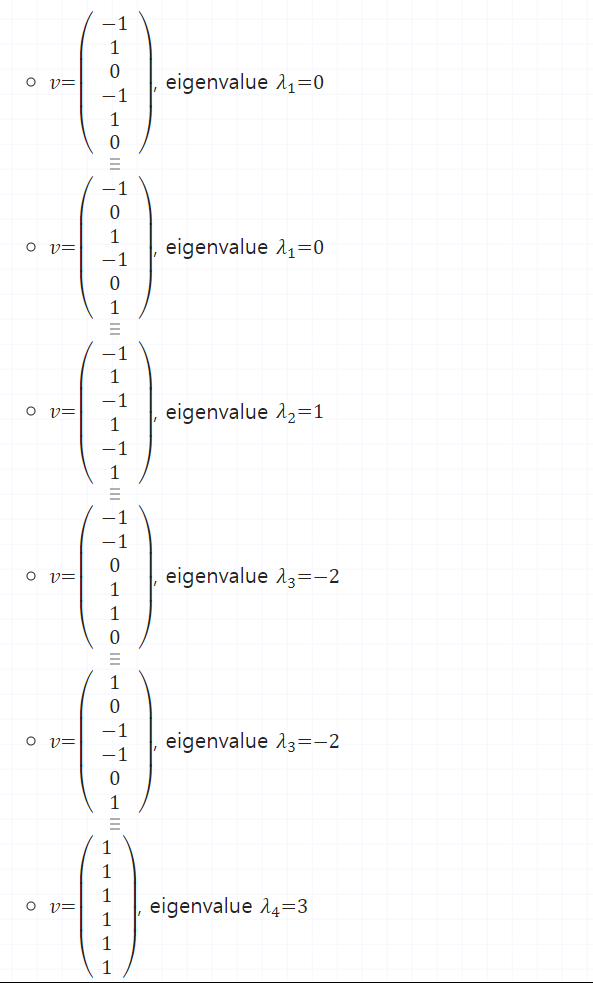
\includegraphics[width=1\linewidth]{image2.png} \\
\end{proof}

\end{document}
